\documentclass{standalone}
% Load any packages needed for this document
\begin{document}

\setcounter{section}{4}
\section{Chapter 5: Hardware for VR}
complete VR installation consists of three main parts:
\begin{itemize}
\item User field: consists of various persons and/or application fields
\item Simulation field: consists of efficient computer(calculates presentation from the virtual environment) and also the feedback from the user
\item Interaction field:interaction field consists of the human-computer interface, which is used for the analog-in and output of the VR data 
\end{itemize}

\subsection{Visual In- and Output Devices}
\begin{itemize}
\item eye is the most important perception channel
\item Active Displays: generate the light for illumination(CRT, LED, VFD, plasma display)
\item use ambient light or background illumination(LCD)
\end{itemize}

\subsubsection{Display Technologies}

\subsubsection*{Cathod Ray Tube(CRT)}
\begin{itemize}
\item Developed by Ferdinand Braun at 1909
\item principle:
	\begin{enumerate}
		\item system heats up the metallic cathode until it will slightly glow
		\item electrons are separated from the metallic structure
		\item positively charged acceleration grid accelerates the electors
		\item most of electrons pass through and reach the focusing unit
		\item in focusing unit, wide electron beam is focused 
		\item deflection unit(capacitor plates or coils) deflects the beam
		\item electrons hit the phosphoric layer and activates the phosphor to emit light (fluorescence)
	\end{enumerate}
\item Note: different kinds of phosphor can be used for different time of persistence (after-glow)
\item For multiple colors, \textbf{penetron tube / mask tube} is used
\begin{itemize}
\item Penetron Tube: works in the same way as cathod ray tube but different floresence colors are stacked at thte inside of the tube. In order to activate different layers, the electrons must have different kinetic energies.
\item Mask Tube: florescence colors are arranged in small triples or stripes(dots are visible if enlarged)
\end{itemize}
\item hole-mask or a slot-mask is used infront of the phosphoric layer which eliminates all unfocused electrons due to its positive charge
\item limitation of resolution is not given by cathod ray-tube but by the image is digitally processed
\begin{itemize}
\item vector technology: pros(no discretization, small amount of memory transformation in hardware) cons(only polygons, no surfaces, only low complexity otherwise image flicker)
\item grid technology: pros(surfaces can be displayed, simple and cheap, complex geometry possible) cons(visible steps, framebuffer needed, scan conversion needed) : ongoing technical development completely replaced by grid technology.
\end{itemize}
\end{itemize}

\subsubsection*{LC Displays}
\begin{itemize}
\item LC: Liquid Crystal in fluid state behaves like a fluid but also show some crystalline properties at the same time.
	\begin{itemize}
		\item Three different states: nematic smectic, cholesteric
		\item LC refracts light $\rightarrow$ depolization
		\item three states
			\begin{itemize}
				\item Nematic: all molecules have the same orientation
				\item smectic state: all molecules have the same orientation but in addition arranged in layers that can be easily displaced againtst each other.
				\item cholesteric state: the crystals are arranged in thin layers which form a helix
			\end{itemize}
	\end{itemize}
\begin{itemize}
\item principle
	\begin{itemize}
		\item voltage $\rightarrow$ LC oriented $\rightarrow$ no refraction $\rightarrow$ light is polarized $\rightarrow$ dark dot (filtered)
		\item no voltage $\rightarrow$ LC not oriented $\rightarrow$ refraction $\rightarrow$ depolarized $\rightarrow$ light dot
	\end{itemize}
\end{itemize}
\item structure:
	\begin{figure}[H]
		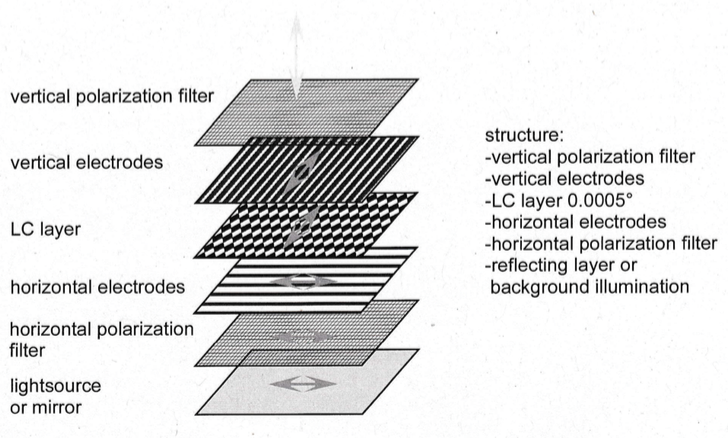
\includegraphics[width=\linewidth]{5_23}
	\end{figure}
\item pros:
	\begin{itemize}
		\item small energy consumption (usually only 20\% of the screen is dark) $\rightarrow$ portable devices
		\item voltage interference (undesirable voltage peack) appears to be dark dot which is less disturbing
	\end{itemize}
\item LCDs have three different groups
\begin{itemize}
\item TN(Twisted Nematic): easiest and cheapest, LCD cells are turned by 90 deg
\item STN(Super Twisted Nematic): twisted by 180 deg and 270 deg. results in a better contrast but results in coloring
\item FSTN(Filmed Super Twisted Nematic): additional thin film layer to improve readability and contrast
\end{itemize}
\item Passive matrix technology vs active matrix technology
\begin{itemize}
\item Passive matrix:
\item active matrix
\end{itemize}
\item color matrix lcds:
\end{itemize}

\subsubsection*{Ferroelectric Liquid Crystal Displays(FLCD)}
\begin{itemize}
\item Liquid crystal displays made out of ferroelecric displays have a much higher switching frequency than nematic LCDs
\item once they are set they remain on the same position
\item \textbf{Pockel Effect}: with an applied voltage field changes refractive index and the crystal is said to be birefringent.(refraction depends on the polarity of the incoming light.
\item To use for light modulation, the crystal is placed between a polarizer and a crossed(90 deg) analyzer.
\item voltage off: the plane-polarized light passes through the crystal, blocked by the analyzer (black)
\item voltage on: crystal becomes more birefringent, light becomes more elliptically polarized (white)
\item only two state (no color, no grayscale) but better contrast 
\item larger display 
\item hard to manufacture and very sensitive
\end{itemize}

\subsubsection*{LED-Screens}
\begin{itemize}
\item LEDs are a semiconductor with long hisory(used from 1960s)
\item used for applications that don't need high resoultion
\item Diode consist of two zones
	\begin{itemize}
		\item overplus electrons arises in one zone while there will be a lack of electrons in the other zone(so-called holes)
		\item when electrons from one zone fill up the holes from the other zone, additional energy is released emitting in the form of light
	\end{itemize}
\item the consistence of the material determines the wavelength of the emitted light. (color)
\item robust and long life cycle
\end{itemize}

\subsubsection*{Plasma Displays(PDP)}
\begin{itemize}
\item A plasma screen is a self-emissive device: using electrodes, a gas is ionized which emits an electro-magnetic radiation. (no background illumination needed)
\item neon, argon, xenon are used (gas is enclosed in small chambers of a glass plate)
\item all electrodes can be addressed individually, every point of the matrix can be activated.
\item the gas has a hystersis effect (right figure)
	\begin{figure}[H]
		\begin{subfigure}[b]{0.45\textwidth}
			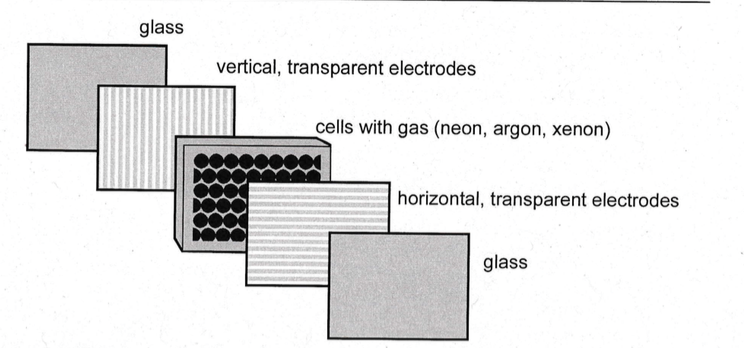
\includegraphics[width=\linewidth]{5_39}
		\end{subfigure}
		\begin{subfigure}[b]{0.45\textwidth}
			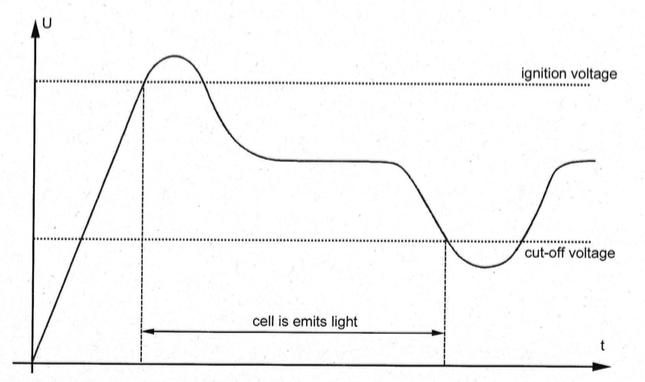
\includegraphics[width=\linewidth]{5_40}
		\end{subfigure}
	\end{figure}
	
	\begin{itemize}
		\item ignition voltage: activate the gas $\rightarrow$ light emission
		\item cut-off voltage: gas stops emitting light
	\end{itemize}
\item pros:
	\begin{itemize}
		\item small dimension in depth
		\item high light intensity
		\item high brilliance in color
		\item brightness and contrast
		\item robust and insensitive to magnetic fields
		\item can be used in large flat screens
	\end{itemize} 
\item cons:
	\begin{itemize}
		\item high energy consumption 
		\item not suitable for high-resolution, small display
	\end{itemize}
\end{itemize}

\subsubsection*{OLED Techonology}
\begin{itemize}
\item OLED is a promising
\item working principle
	\begin{itemize}
		\item double bond in the benzene ring opens by adding a small amount of energy (source of free electron: pi-electron)
		\item on: from the structure, pi-electron can be lifted to a higher trajectory 
		\item off: electrons fall back to a lower trajectory and emitting light
		\item by changing material, different color of light can be produced
	\end{itemize}
\item cheap and better read-out angle compared to LCD. (no background light, emitting light directly)
\item bright, good contrast and good read-out angle
\item short life cycle and weak to the water or oxygen
\item OLEDs age if they are not switched on (loss of color)
\item subgroups derived:
	\begin{itemize}
		\item TOLED(Transparent Organic Light Emitting Diode): highly transparent (can be applied to windows)
		\item SOLED(Stacked Organic Light Emitting Diode): stacked film for RGB. Higher resolution than other displays.
		\item FOLED(Flexible Oranic Light Emitting Diode): can be bent with a radius down to 6 mm 
	\end{itemize}
\end{itemize}

\subsubsection*{Field Emission Display}
\begin{itemize}
\item similar working principle with CRTs but electrons are emitted from thousands of small metallic micro tips: one micro tip per pixel
\item by applying a voltage between the micro tips and the phosphoric screen, the electrons are emitted. 
\item as electrons hit the phosphoric layer, light is emitted (\textbf{field emission})
\item material for micro tips:
	\begin{itemize}
		\item tradition: tapered metallic electrodes
		\item no heating system is needed (instead, high voltage is needed)
		\item carbon, diamond have the field emission effect at lower voltage 
	\end{itemize}
\item thin, low power consumption but viewing angle and the colors are similar to CRT
\end{itemize}

\subsubsection*{Electronic Paper}
\begin{itemize}
\item a layer is small capsules with 100 um in diameter between two electrodes. 
\item pigments have a positive(white) or a negative(black) charge. 
\item depending on the applied voltage of electrodes the white or black pigments move to the surface of the capsule and generate a black or a white pixel. 
\item pigments stay at the location even if the voltage is switched off 
\item almost every surface can be used as a display
\end{itemize}

\subsubsection*{Comparison between the Different Technologies}
\textbf{See 5.1.1.14 page 5-41}

\subsubsection{Projectors}

\subsubsection*{Tube Projectors(CRT Projectors)}
\begin{itemize}
	\item uses a cathode ray tube for every basic color (red, green, blue)
	\item images are added on the screen using \textbf{additive color model}
	\item extensive adjusting procedures are necessary: because all three colors are projected individually, adjust all colors precisely at the same location on the screen (if not, blurred image)
	\item image distortion
		\begin{itemize}
			\item horizontal distortion: due to misalignment between each colored images $\rightarrow$ solution: additional lenses
			\item vertical distortion(``keystone effect"): height of the projector is not adjusted property (or mounted on the ceiling) $\rightarrow$ solution: additional optics or electronically
		\end{itemize}
	\item drawback: limited maximum amount of emitted light (10 times less than DLP or LC projector)
\end{itemize}

\subsubsection*{DLP Projectors}
\begin{itemize}
	\item Digital Mirror Device(DMD) is the main part in a DLP Projector, which is an array of adjustable small mirrors that can be addressed by pulse-width-modulation in a digital way (one mirror for every pixel)
	\item DMD can switch on and off the incoming light (by electrostatic attraction)
		\begin{itemize}
			\item 1: $\rightarrow$ twists toward lens
			\item 0: $\rightarrow$ twists toward absorber
		\end{itemize}
	\item greyscales are realized by a \textbf{binary pulse-width modulation}(4-bit sequence) of the incoming light
		\begin{itemize}
			\item if changes in brightness are too fast, the human eye will integrate - high frequency $\rightarrow$ brighter
			\item 4 bit sequence - 0/15 $\sim$ 15/15 (brightness level)
		\end{itemize} 
	\item DMD is expensive in manufacturing $\rightarrow$ should be optimally used
	\item color: available DLP projectors can be distinguished into 1, 2, or 3 chip projectors
		\begin{itemize}
			\item 1 chip DLP: one DMD for 3 colors
			\begin{itemize}
				\item white light is dispersed into red, green and blue using a rotating wheel with color filters (processed serially)
				\item usually a white segment is used to assist in boosting lumens projected onto the screen
				\item rainbow effect: (drawback) if rapid movements combined with high contrasts, three basic colors can still be seen. (faster spinning color wheel or wheel with more segments needed)
				\item additional draw back is that the amount of light per color is only one third
				\item alternative: SCR DLP(Scrolling Color Recapture or Sequential Color Recapture)
					\begin{itemize}
						\item light source + focusing unit + light integrator + SCR wheel + DMD
						\item made out of a material with dichroitic properties and reflects the amount of light that cannot pass through into the light integrator
						\item light integrator is used to bundle the light
						\item in order to provide all basic colors on the chip simultaneously and within the light integrator as well, the colors of the color wheel are arranged in a so-called archimedes shape					
					\end{itemize}
			\end{itemize}
			\item 2 chip DLP
			\begin{itemize}
				\item A color wheel disperes the incoming light into \textbf{yellow} and \textbf{magenta} which are given to a color-seperating prism afterwards
				\item The color prism seperates magenta into red and blue, while yellow will be dispersed into red and green
				\item Since red is a relevant part after each dispersion, it is not time-multiplexed and thus needs a seperate DMD
				\item Green and blue are time-multiplexed and thus can share another DMD that is synchronized with the colorwheel
			\end{itemize}
			\item 3 chip DLP
			\begin{itemize}
				\item A prism disperses the white light into the colors red, green, and blue which are reflected individually by the DMD-chips
				\item Expensive, thus used in professional installations
			\end{itemize}
		\end{itemize}
	\item color depth of 24 bit (8 bit for each color)
	\item optical efficiency of the DLP projection system: $ \text{Lamp} \times \text{colorfilter} \times \text{pixel} = total$
\end{itemize}

\subsubsection*{LC Projectors}
\begin{itemize}
\item LC projectors can be subdivided into single and triple chip projectors
\item In a LC projector, the image is generated on three LC panels for red, green and blue
\item create color digitally (color pallette)
\item pros:
	\begin{itemize}
		\item easy handling: no adjustment of convergence is needed (only one lens)
		\item high brightness
	\end{itemize}
\end{itemize}

\subsubsection*{LED Projectors}
\begin{itemize}
\item small projectors
\item like a normal DLP, but light source is LED

\end{itemize}

\subsubsection{Stereo Display Technologies}
\begin{itemize}
	\item The devices described previously can only project 2D images
	\item Stereo Display Technology allows using the display technology as described so far also for a real stereoscopic display of objects
	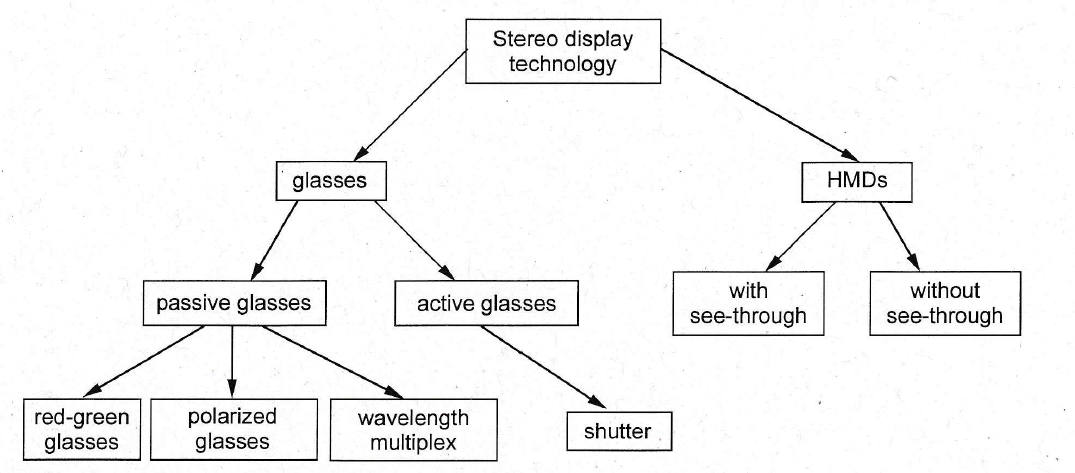
\includegraphics[scale=0.5]{5_103}
	
	\item Passive Red-Green Glasses (Anaglyphe Technology)
	\begin{itemize}
		\item Visualization devices produce two images, projected at the same time in red and green
		\item The two images are almost identical but slightly displaced towards each other by the amount of the horizontal parallax(eye distance)
		\item The image is viewed through filters, red filter in front of one eye and green filter in front if the other(with bare eyes the image appear blurred)
		\item Eyes see a slightly different image due to the parallax, resulting in a stereoscopic image
		\item Drawback: only red and green images can be generated, which appear monochrome when wearing the glasses \\
		if other colors are used the stereoscopic effect is destroyed
		\item Advantage: cheap installation of the system
	\end{itemize}

	\item Polarized Glasses (Linearly)
	\begin{itemize}
		\item A stereoscopic image with full colors can be generated since the polarization filters do not filter out any specific frequencies
		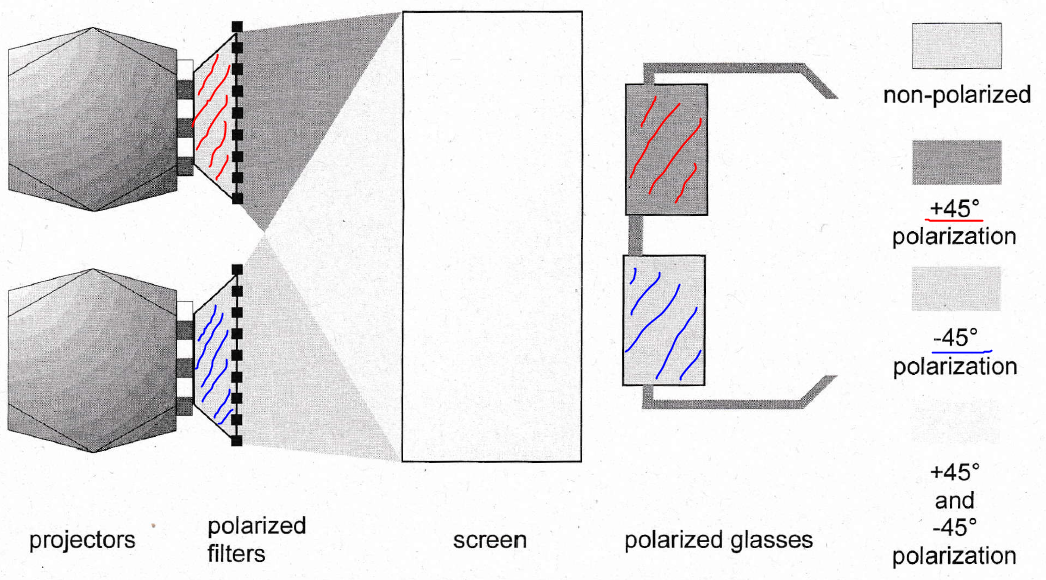
\includegraphics[scale=0.4]{5_106}
		\item z-screen: Today, using only one projector is possible but with an additional polarization filter that can be electrically switched
			\begin{itemize}
				\item however this results in a change from a parallel projection of the two required channels to a serial projection, which requires projectors that can switch fast enough
			\end{itemize}
		\item Advantages
			\begin{itemize}
				\item color images can be displayed 
				\item Glasses have a low transmission loss and thus the images stay bright
				\item Moving pictures can be displayed with the maximum image repetition frequency available from the projectors
				\item Filters and glasses are inexpensive
			\end{itemize} 
		\item Drawback
			\begin{itemize}
				\item two projectors(or one projector with a z-screen) are needed, as well as a specially coated screen that doesn't change the polarization between the incoming and the reflected light
				\item Linear polarization causes losses
				\begin{itemize}
					\item Transmittance of the polarization filter is defined as K and is between a maximum value k\textsubscript{2} and a minimum value  k\textsubscript{1}
					\item if a polarization filter is placed in front of a projector that emits unpolarized light: $ K = \frac{ k\textsubscript{2} + k\textsubscript{1}}{2} $
					\item two filters (projector and eye) polarized in the same direction: $ H\textsubscript{0} = \frac{ k\textsubscript{2}^2 + k\textsubscript{1}^2}{2} $
					\item if the orientations of the two filters are perpendicular to each other: $ H\textsubscript{90} = k\textsubscript{2}*k\textsubscript{1} $ 

					\begin{figure}[H]
						\centering
						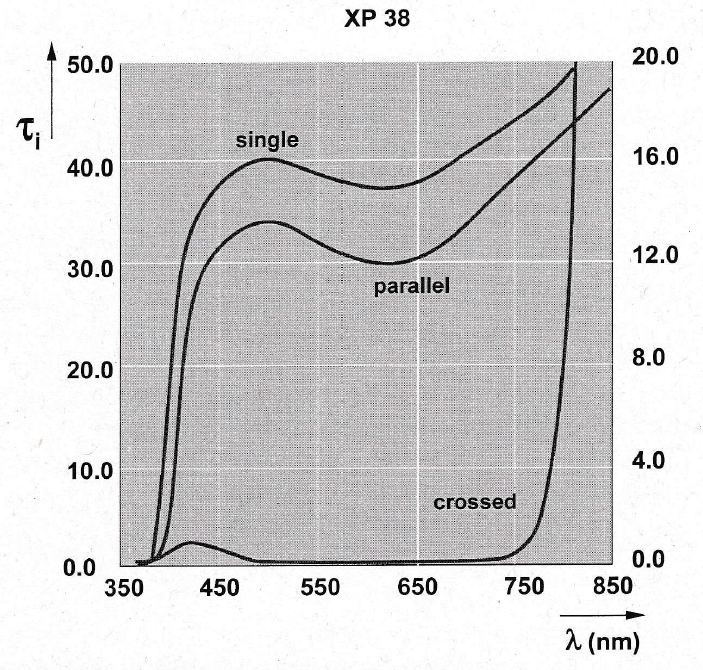
\includegraphics[scale=0.25]{5_108}						
					\end{figure}

					\item the lower curve is also called "leakage"
					\item Problem: \textbf{the alignment of the filters depends on the posture or on the head tipping of the audience}; even small rotations of the head lead to a significantly increased leakage or crosstalk(sometimes called ghosting) 
					\item relationship between the angle $\theta$ and the transmittance: $ K = (k\textsubscript{1}-k\textsubscript{2})*\cos ^2(\theta)+k\textsubscript{2} $ 
				\end{itemize}
			\end{itemize} 
	\end{itemize}
	
	\item Polarized Glasses (Circular)
	\begin{itemize}
		\item The superposition of two linearly polarized waves, which are orthogonal to each other and which have a phase shift of 90$^{\circ}$, results in a circularly polarized wave
		\item If two sinusoidal oscillations with the same amplitude are superimposed, the E-vector does not oscillate anymore within the plane, but rotates around the z-axis \\
		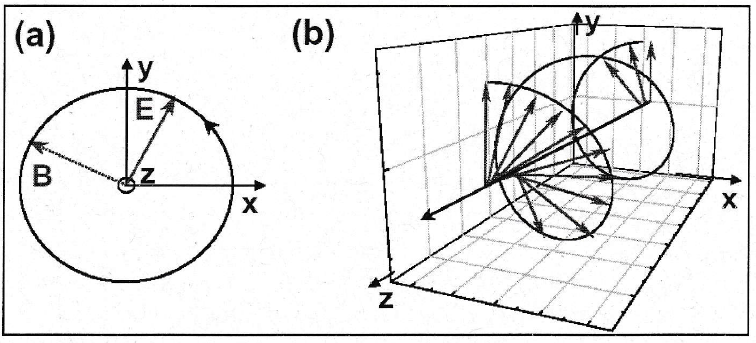
\includegraphics[scale=0.5]{5_112}
		\item The set-up for generating circularly polarized light consists of a filter for linear polarization and a quarter-wavelength retarder \\
		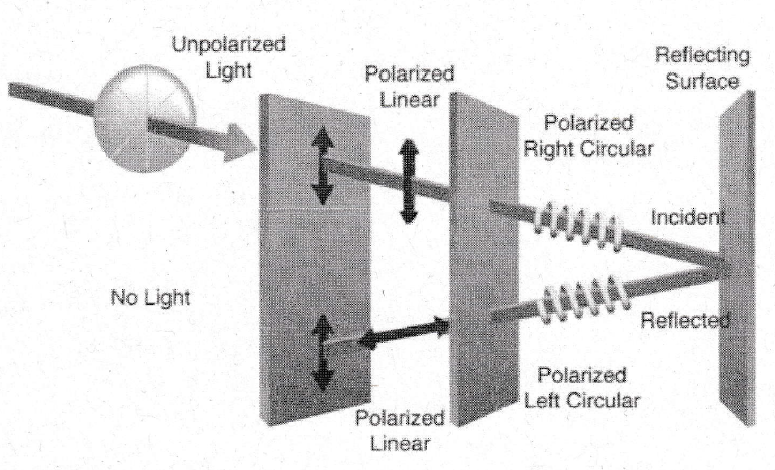
\includegraphics[scale=0.5]{5_113}
		\item Retarder: to transform linearly polarized light into circularly polarized light) \\
		consists of a material that retards the incoming light depending on the polarization due to multiple reflections in the material \\
		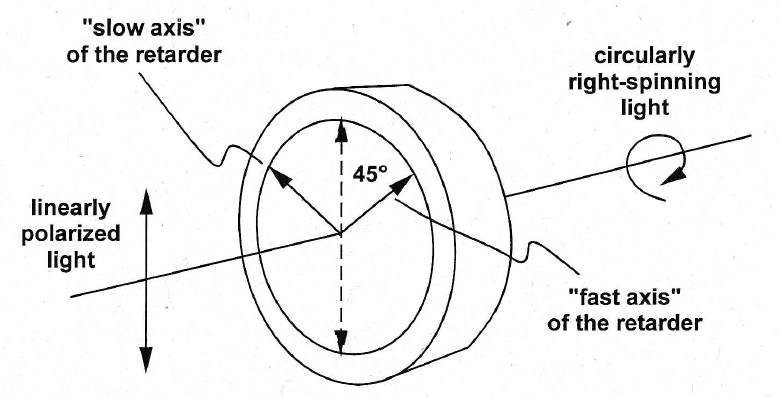
\includegraphics[scale=0.4]{5_114}
		\item The linear polarization of the incoming light has an angle of 45$^{\circ}$ to the slow axis and to the fast axis as well and is thus divided into two identical parts. Between the fast and the slow axis, there is a runtime difference of $\frac{\lambda}{4}$ for a given wavelength. The superposition of both light paths gives the wanted circular polarization
		\item The wave changes its spin orientation and reaches the user by the reflection on the screen. The
user wears glasses with another retarder and a polarization filter. The retarder converts the circularly polarized light into light with linear polarization.
	\end{itemize}
	
	\item Shutter Glasses
	\begin{itemize}
		\item The image on the visual output device is changed periodically, and an image for the left and the right eye is displayed alternately(two images are slightly different from each other due to the eye distance)
		\item The user wears shutter glasses, which are synchronized with the displayed images and alternately darken the left and the right eye
		\item Thus, every eye has a certain perspective and the stereoscopic sensation arises
		\item An infrared emitter sends synchronization pulses to the glasses which work with the typical LC-principle
		\item Advantage: low cost of the overall system
		\item Drawback: the user has to turn his head towards the monitor or the screen all the time(because otherwise infrared link cannot synchronize) \\
		the active shutter glasses are rather expensive
		\item When displaying active stereo images on normal TV sets, the even lines are used for the left eye while the odd lines are used for the right eye
	\end{itemize}
	
	\item Head Mounted Display (HMD)
	\begin{itemize}
		\item The idea of HMD is based on a stereoscope
		\item Advantage: the natural head movements are not restricted, so the user can freely explore by moving around and watching from different positions
		\item Drawback: heavy weight of the device, relatively small field of view(FOV)
		\item In order to address the two displays of an HMD, typically two graphics cards are needed but also possible to use only one graphics card by applying 'field-sequential procedure' or 'interlaced procedure' 

		\begin{figure}[H]
			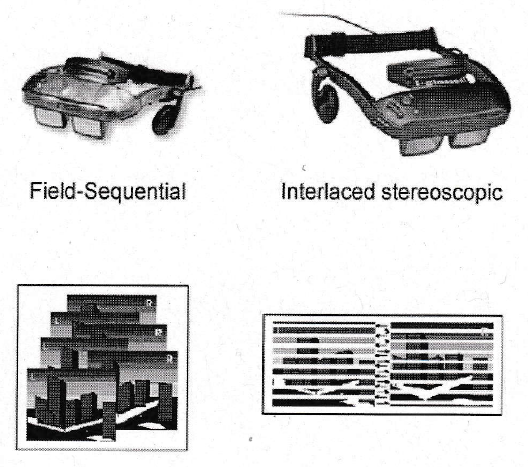
\includegraphics[scale=0.6]{5_120}			
		\end{figure}
		
		\begin{itemize}
			\item field-sequential procedure: reduces the image repetition frequency by half, Interlaced procedure reduces the image resolution by half
			\item interlaced procedure: the number of lines of an image is halved. (one for left, one for right)
		\end{itemize}
		
		\item Angular resolution is one way to compare the perceived image quality - takes 2 factors into account:
		\begin{itemize}
			\item The horizontal and vertical resolution of the internal display system(CRT or
LCD) in pixels
			\item The horizontal field of view(FOV) in degrees
		\end{itemize}
		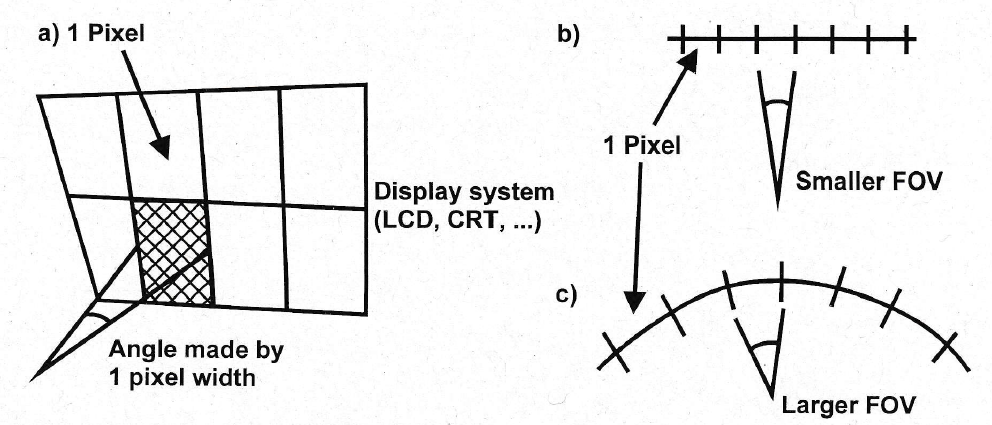
\includegraphics[scale=0.4]{5_121}
		
		\item FOV is hard to measure since there exists no standard method \\
		the main reason for the large variations is that some HMDs only allow a monoscopic display while others allow a stereoscopic vision(In case of a stereoscopic vision, the two displays must overlap which means FOV is limited and could be very small)
		\item Even though 20 percent of FOV being the central stereopsis region(overlap) is sufficient to give the user a good sense of depth, the overlap region is set to a greater value to provide a safety margin in case the user's gaze changes; the regions of overlap are very different depending on the devices
	\end{itemize}
	
	\item 3D Displays, Autostereoscopic Displays
	\begin{itemize}
		\item For autostereoscopic displays, the users don't have to wear special devices
		\item classification
			\begin{itemize}
				\item projective procedures
				\item volumetric procedures
			\end{itemize}
		\item projective procedures
			\begin{itemize}
				\item Parallax Barriers
					\begin{itemize}
						\item a vertical grid of one pixel in width, which generates small barriers that block the view onto the display behind 
						\item mask blanks the even columns for the right eye and the odd columns for the left eye by barrier
						\item due to the small size of the blanked pixel columns, the visible system does not recognize the mask and generates a three-dimensional scene out of the two perceived images 
						\item This procedure can also be used for the generation of more than two independent views by varying the distance and the width of the parallax barriers
					\end{itemize}
				\end{itemize}	
				
				\begin{figure}[H]
					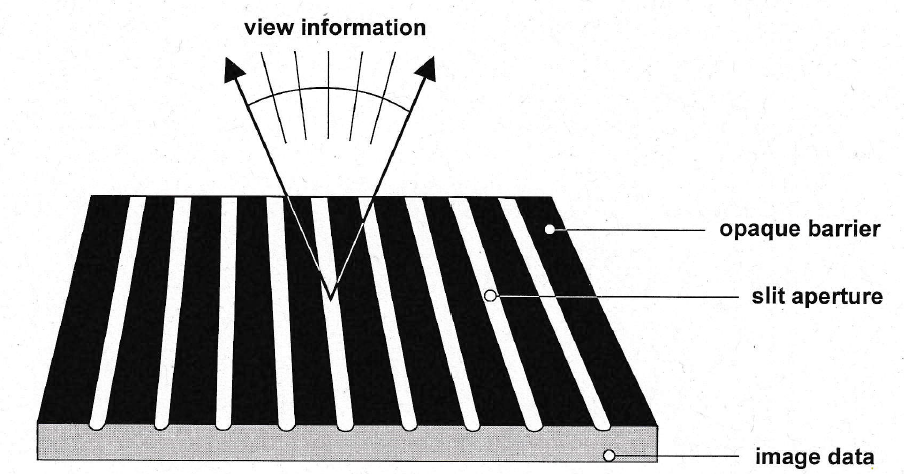
\includegraphics[scale=0.4]{5_126} 					
				\end{figure}

		\item Lenticular Lenses
			\begin{itemize}
				\item a layer of vertical semi-cylindrical lenses can be used to display adjacent pixels separately and to project them into the room
				\item very similar to the method of parallax barriers, but the lenticular lenses do not allow any direct view onto the pixels of the LC-display; only the amount of light is visible to the user that is refracted in direction of the actual eye position 
				\item the lens array consists of a glass pane with a large amount of micro lenses 
				\item Behind the lens array, two stereoscopic semi-images are displayed(odd columns for the right eye and even columns for the left eye); the computer has to generate two different signals for the displays, which will be combined by a multiplexer in an alternating way 
				\item The stereoscopic sensation depends on the head position of the user, so the 3D display systems have an automatic adjusting system which adapts the monitor to the head movements 
				\item A video camera takes an image of the user's eye distance, making it possible to readjust the position of the lens array
				\item Drawback: the user has to be at an exactly defined position(but multiple users are possible)
			\end{itemize} 

		\begin{figure}[H]
			\begin{subfigure}[b]{0.45\textwidth}
				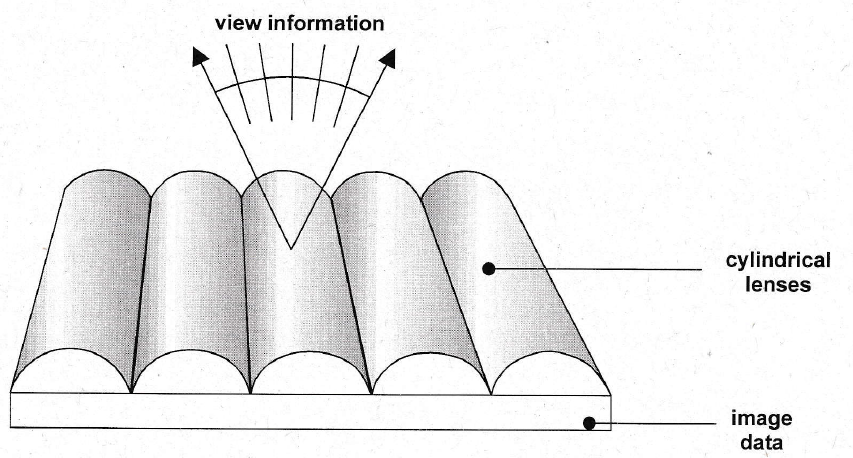
\includegraphics[width=\linewidth]{5_127} 
			\end{subfigure}
			\begin{subfigure}[b]{0.45\textwidth}
				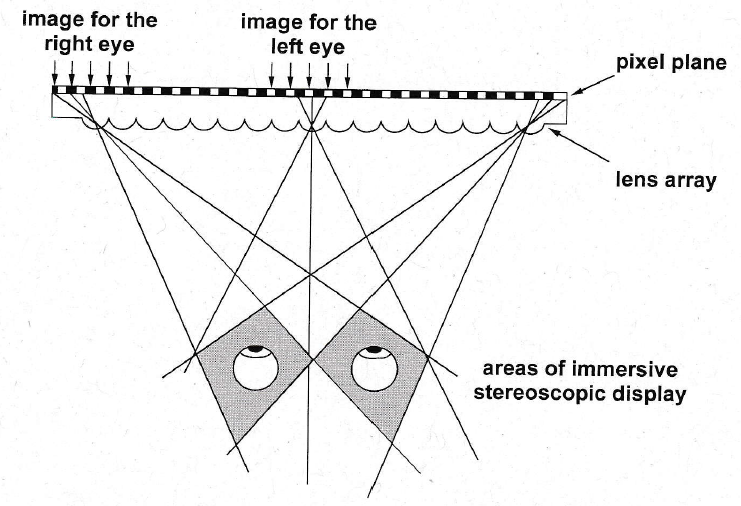
\includegraphics[width=\linewidth]{5_128}
			\end{subfigure}
		\end{figure}

		\item Integral Imaging
			\begin{itemize}
				\item an array of hemispheric lenses results instead of lenticular lenses 
				\item high-resolution images and allowed stereo- and motion parallaxes into all directions within a certain range
			\end{itemize}
			
			\begin{figure}[H]
				\centering
				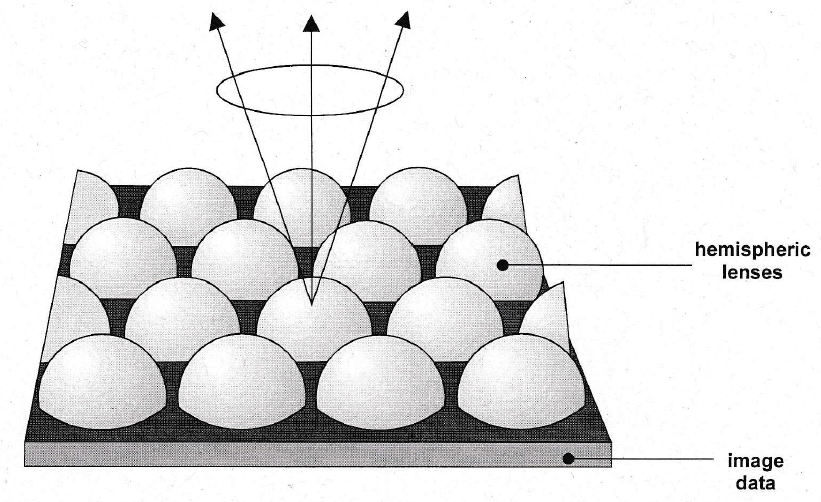
\includegraphics[scale=0.35]{5_131} 
			\end{figure}
			
		\item Volumetric Displays
			\begin{itemize}
				\item Volumetric procedures distinguish from the projective procedures by the way points in space are addressed (projective displays only throw pre-calculated perspective images into space)
				\item volumetric displays directly define each pixel within the projection volume with regard to its intensity and color 
				\item e.g. Actuality Systems: a laminated helix rotates inside a glass sphere with such a high rotation speed that the helix becomes almost invisible. The required pixels in space are illuminated by three color lasers at that moment, when the surface of the helix is at the right location(below left)
			\end{itemize}
		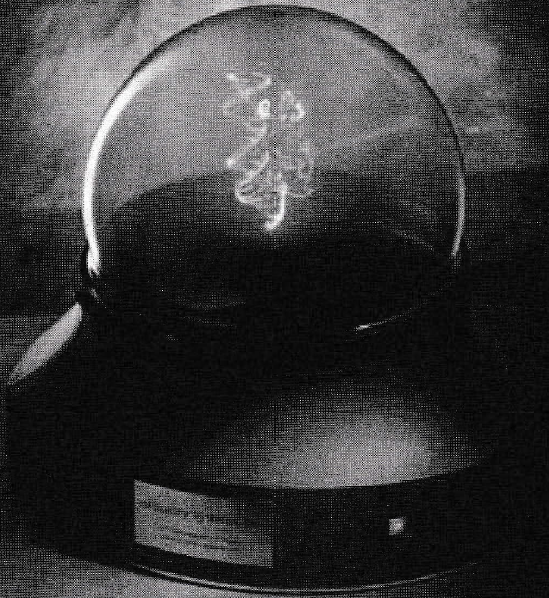
\includegraphics[scale=0.3]{5_133} 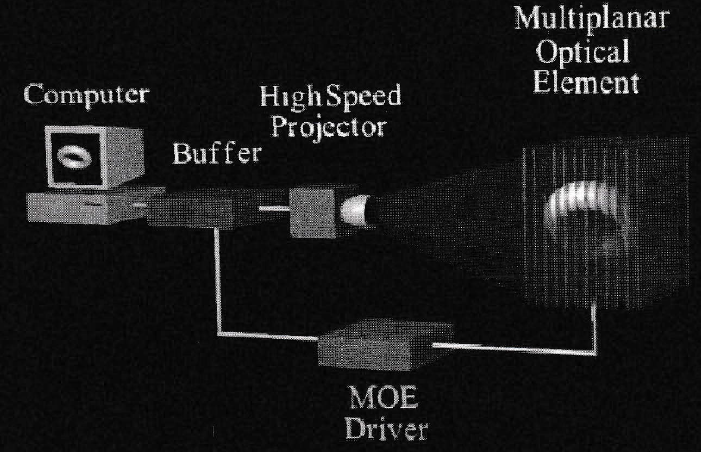
\includegraphics[scale=0.4]{5_134}

		\item DepthCube
			\begin{itemize} 
				\item based on a back projection system 
				\item two main components:
					\begin{itemize}
						\item a high-speed video projector 
						\item multiplanar optical element, in which each slide defines a certain depth 
					\end{itemize}  
				\item all pixels are really projected onto different locations in the projection space; the user has an impression of depth by accommodation and by convergence as well
			\end{itemize}
	\end{itemize}
	
	\item Wavelength Multiplex Systems ``Infitec"
	\begin{itemize}
		\item The perception of visible information is performed by receptors, which have different sensitivities to different colors
		\item It uses the fact that image information can be transmitted in parallel in slightly different wavelength triples(color values). The complete image information is split into two channels by this color separation
		
		\begin{figure}[H]
			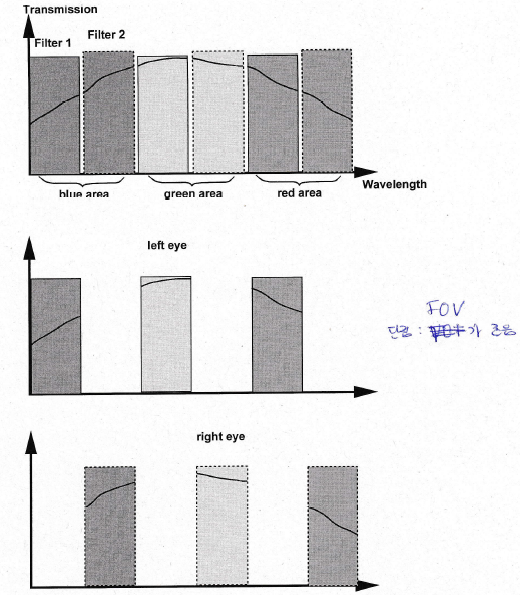
\includegraphics[scale=0.7]{5_136}			
		\end{figure}
		
		\item Two projectors are required, each of them equipped with a special filter to perform a specific color shift
		\item Optical notch filters(realized by multi-layer dielectric coating onto a suitable carrier material) are needed to separate the content for left and right eye
		\item By increasing the amount of resonators in the optical notch filters, the quality and selectivity of the filter can be increased which determines the amount of parallel channels for transmitting the image content
		\item Advantage: 
			\begin{itemize}
				\item a complete RGB-system per eye is available 
				\item exists a possibility for simultaneous visualization of multiple, stereoscopic perspectives for more than one user 
				\item the projection can also be performed in rooms with ambient light without any loss in contrast since the separation of different images is done by filters that have a very small optical bandwidth
			\end{itemize}
		\item Constraint: all spectral frequencies are within the bandwidth of activation for one certain color receptor
	\end{itemize}		
\end{itemize}

\end{document}